\subsection{RQ3: Retrieval, Toolkit Quality and Certification}
\label{sec:ev-rq3}

RQ3 asks whether reasoning over typed capabilities finds better toolkits than retrieval alone. We separate three
levels that are often conflated: finding the right single tool (retrieval quality), exposing a small set that
covers a multi-step task (gold-tool recall at a given size), and exposing a set whose interfaces, effects and
flows are jointly feasible (functional sufficiency, checked by an evaluator independent of the certificate).
Executed task success is not measured (Fig.~\ref{fig:ev-evidence}).

\emph{Protocol.} Retrieval is measured on the 300 test requests against benchmark gold (measured), over the 81
MCPToolBench++ tools and over the full registry; every method, including thirteen ranking variants of \pamcp{},
was configured on the 60 development requests only, and the selection rule was fixed before the test run. The
variants isolate the components of Eq.~(5) (lexical, dense, structural), relevance-first orderings,
confidence-gated or down-weighted structural matching, and oracle types (goal output types or tool output types
replaced by $J_B$), which are diagnostic and not selectable. Toolkits are built for the 94 LiveMCPBench test
tasks; group recall counts a task's gold steps (alternative tools of one step count once). Joint feasibility is
decided by two independently written evaluators that use $J_B$ and the analyst's goals: a coarse one that
compares output kinds and effect classes, and a strict one that also compares domains and collection cardinality,
derives required inputs from the schema and treats any egress of private data as a flow violation.

\begin{table}[t]
\centering
\caption{Single-tool retrieval on the 300 test requests with configurations selected on the development split:
Hit@1 over the 81 MCPToolBench++ tools and, with target-tool clustered 95\% CI, over the 569-tool registry, and
the other metrics over 569 tools.}
\label{tab:ev-retrieval}
\scriptsize
\setlength{\tabcolsep}{2.4pt}
\begin{tabular}{@{}lrrrrrr@{}}
\toprule
 & 81 tools & \multicolumn{5}{c}{569 tools} \\
\cmidrule(lr){2-2}\cmidrule(l){3-7}
Method & Hit@1 & Hit@1 [CI] & Hit@3 & Hit@5 & MRR & nDCG \\
\midrule
BM25 & 52.7 & 41.0 [26, 60] & 57.3 & 63.7 & 0.503 & 0.543 \\
RAG-MCP (dense) & 49.7 & 37.3 [22, 56] & 50.0 & 54.3 & 0.451 & 0.492 \\
RRF fusion & 54.3 & 38.7 [23, 57] & 54.7 & 61.3 & 0.481 & 0.525 \\
MCP-Zero & 68.0 & 66.7 [49, 80] & 80.0 & 85.7 & 0.743 & 0.775 \\
COLT & 49.7 & 37.3 [22, 56] & 50.0 & 54.3 & 0.451 & 0.492 \\
ToolScope & 53.0 & 41.0 [26, 60] & 58.3 & 63.7 & 0.504 & 0.543 \\
CMTF & 58.7 & 32.7 [19, 49] & 47.0 & 54.7 & 0.428 & 0.488 \\
PaMCP (Eq. 5) & 61.0 & 29.7 [16, 47] & 45.7 & 53.7 & 0.400 & 0.461 \\
PaMCP-L & 72.0 & 41.3 [25, 60] & 61.3 & 69.3 & 0.536 & 0.603 \\
PaMCP, oracle types (diag.) & 71.7 & 58.3 [38, 74] & 75.3 & 81.3 & 0.680 & 0.728 \\
\bottomrule
\end{tabular}
\end{table}


\begin{figure*}[t]
\centering
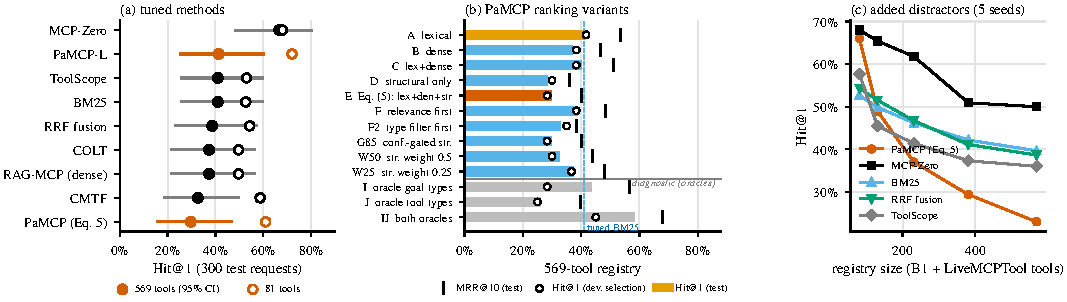
\includegraphics[width=\textwidth]{fig_rq3_retrieval}
\caption{Single-tool retrieval (300 test requests). (a) Hit@1 of the tuned methods over 81 and 569 tools
(target-tool clustered 95\% CI). (b) \pamcp{} ranking variants over 569 tools: test Hit@1 (bars), test MRR@10
and the development Hit@1 used for selection; oracle rows are diagnostic. (c) Hit@1 as LiveMCPTool tools are
added to the 81 MCPToolBench++ tools (protocol scoring, five seeds).}
\label{fig:ev-retrieval}
\end{figure*}

\emph{Retrieval: structural matching hurts at scale unless typing is right.} Over the 81 MCPToolBench++ tools
the relevance-first variant \pamcp{}-L ranks the gold tool first for 72.0\% of the requests and the original
ranking of Eq.~(5) for 61.0\%, against 68.0\% for MCP-Zero and 49.7--58.7\% for the other baselines
(Table~\ref{tab:ev-retrieval}). Over 569 tools the ordering changes: MCP-Zero, whose requests are written by the
model for routing, reaches 66.7\% (95\% CI 48.6--80.2\%), \pamcp{}-L 41.3\%, tuned BM25 and ToolScope 41.0\%, and
Eq.~(5) only 29.7\%, the lowest of the tuned methods (Fig.~\ref{fig:ev-retrieval}a). The loss grows with every block of added
tools (Fig.~\ref{fig:ev-retrieval}c). The variants locate the cause (Fig.~\ref{fig:ev-retrieval}b): structural
ranking alone reaches 28.3\%, and adding it to lexical and dense ranking lowers Hit@1 from 40.0\% to 29.7\%;
down-weighting it (0.25) or applying it after relevance recovers most of the loss (37.3\% and 38.7\%), while using
it as a filter first does not (33.0\%). Confidence gating changes nothing, because every gold tool is typed with
confidence of at least 0.85: the typing is confidently wrong at the domain level (Section~\ref{sec:ev-rq1}).
Oracle types show what correct typing would buy: correct goal types alone raise Eq.~(5) to 43.7\%, correct tool
types alone do not help (26.0\%), and both together reach 58.3\%, above every baseline except MCP-Zero. The
dev-selected \pamcp{}-L is not better than tuned BM25 (confirmatory H1: $+0.3$ points, $p_{\mathrm{Holm}}=1.0$)
and its gain over Eq.~(5), $+11.7$ points (95\% CI 3.0--22.6), is not significant after correction (H2:
$p_{\mathrm{Holm}}=0.070$).

\begin{table}[t]
\centering
\caption{Toolkits on the 94 LiveMCPBench test tasks: size, manifest tokens, group recall (task bootstrap 95\%
CI), share of toolkits jointly feasible for the coarse and the strict independent evaluator (least-privilege
policies), and abstentions. Baselines restricted to eligible tools unless marked published.}
\label{tab:ev-sets}
\scriptsize
\setlength{\tabcolsep}{2.1pt}
\begin{tabular}{@{}lrrlrrr@{}}
\toprule
 & & & & \multicolumn{2}{c}{Joint feas. (\%)} & \\
\cmidrule(lr){5-6}
Method & $|K|$ & Tok. & Group recall [CI] & coarse & strict & Abst. \\
\midrule
\pamcp{} ($K{=}10$) & 1.46 & 198 & 0.174 [0.12, 0.23] & 67.0 & 27.7 & 7.4 \\
\pamcp{}-L & 1.22 & 146 & 0.161 & 54.7 & 15.8 & 9.5 \\
\pamcp{} NoCert & -- & -- & -- & 59.6 & 13.8 & 0.0 \\
Per-subtask (elig.) & 2.59 & 346 & 0.249 [0.19, 0.32] & 62.8 & 8.5 & -- \\
RAG-MCP@5 (elig.) & 5.00 & 1244 & 0.293 [0.22, 0.37] & 60.6 & 5.3 & -- \\
COLT@5 (elig.) & 5.00 & 1094 & 0.295 [0.23, 0.37] & 59.6 & 8.5 & -- \\
ToolScope@5 (elig.) & 5.20 & 976 & 0.361 [0.29, 0.44] & 73.4 & 11.7 & -- \\
MCP-Zero (elig.) & 1.76 & 250 & 0.227 [0.17, 0.29] & 57.4 & 11.7 & -- \\
CMTF (elig.) & 0.64 & 105 & 0.072 [0.04, 0.11] & 25.5 & 14.9 & -- \\
RAG-MCP@5 (published) & 5.00 & 1244 & 0.293 [0.22, 0.37] & 48.9 & 5.3 & -- \\
\bottomrule
\end{tabular}
\end{table}


\begin{figure*}[t]
\centering
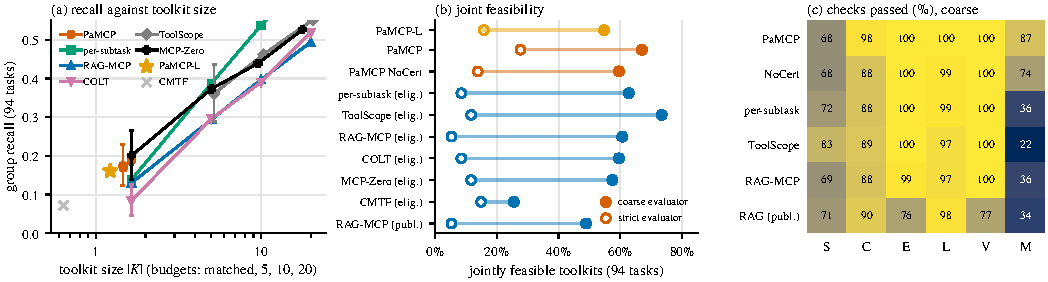
\includegraphics[width=\textwidth]{fig_rq3_sets}
\caption{Toolkits on the 94 test tasks. (a) Group recall against toolkit size for candidate budgets (size-matched,
5, 10, 20; bar: 95\% CI at the smallest budget). (b) Jointly feasible toolkits for the coarse and the strict
evaluator, least-privilege policies. (c) Pass rates of the coarse evaluator's checks: goals served (S), inputs
obtainable (C), effects (E), flows (L), evidence level (V) and minimality (M).}
\label{fig:ev-sets}
\end{figure*}

\emph{Toolkit size and recall.} \pamcp{} exposes 1.46 tools and 198 tokens per task and reaches a group recall of
0.174 (Table~\ref{tab:ev-sets}); methods that expose more tools reach more gold steps: per-subtask retrieval 0.249
with 2.59 tools, RAG-MCP and COLT 0.293 and 0.295 with five tools and more than 1,000 tokens, ToolScope 0.361
with 5.20 tools. Fig.~\ref{fig:ev-sets}a shows that recall is mostly a function of size: at the same size (1.64
tools) \pamcp{} reaches 0.189 against 0.130 for RAG-MCP, 0.138 for per-subtask retrieval, 0.084 for COLT and
0.200 for MCP-Zero, a difference to RAG-MCP that is not significant (F2: $\Delta=0.060$,
$p_{\mathrm{Holm}}=0.397$). Non-inferiority of recall to per-subtask retrieval is not established, neither for
\pamcp{} (F1: $\Delta=-0.080$, 95\% CI $[-0.166, 0.002]$) nor for \pamcp{}-L (H3: $\Delta=-0.088$).

\emph{Joint feasibility and certification.} Under the coarse evaluator, 67.0\% of \pamcp{}'s toolkits are jointly
feasible; it certifies 92.6\% of the tasks and abstains on the rest. Baselines restricted to eligible tools reach
57.4--73.4\% (ToolScope highest, CMTF 25.5\%), and the difference to per-subtask retrieval is not significant (F3:
$\Delta=0.043$, $p_{\mathrm{Holm}}=1.0$). The coarse evaluator is, however, too permissive: on ten hand-built
cases with ground truth fixed beforehand (same JSON shape with another meaning, domain mismatch, missing required
field, array against scalar, scope mismatch, unmet prerequisite, indirect egress of private data, invalid
declassification, conditional dependency, a policy violated only by a pair of tools), it decides 2 correctly and
the strict evaluator 7; the three remaining cases need scope, credential or declassification information that the
labels do not contain. Under the strict evaluator, 27.7\% of \pamcp{}'s toolkits are jointly feasible against
5.3--14.9\% for the eligible baselines and 13.8\% without certification (Fig.~\ref{fig:ev-sets}b; exploratory).
Certification acts through obtainable inputs and minimality (coarse C from 88.3\% to 97.9\%, M from 74.5\% to
87.2\%, against 36\% and 22\% for RAG-MCP and ToolScope; Fig.~\ref{fig:ev-sets}c); the binding constraint under both
evaluators is goal service (S: 68\% coarse, 33\% strict), i.e.\ typing again. The relevance-first \pamcp{}-L does
not improve composition (recall 0.161, strict feasibility 15.8\%; H4 against per-subtask retrieval: $+7.4$
points, $p_{\mathrm{Holm}}=0.277$).

\emph{Interpretation.} Set-level reasoning yields small, certified toolkits whose joint feasibility is higher than
that of retrieval baselines under a strict independent check, but it does not find more gold tools at equal size,
and structural matching lowers single-tool retrieval on the full registry. The oracle results show that the
mechanism is not the bottleneck: with correct goal and tool types the structural ranking would be the second best
retriever. Typed composition is therefore only as good as the typing it consumes, and the evidence supports
\pamcp{} as a pre-execution feasibility filter, not as a superior retriever. Both evaluators consume LLM labels;
neither replaces executing the toolkits.
